\documentclass[aoas]{imsart}
%% LaTeX 2e style file for the processing of LaTeX2e files
%% of the following IMS/BS journals:
%%
%% - The Annals of Probability
%% - The Annals of Applied Probability
%% - The Annals of Statistics
%% - The Annals of Applied Statistics
%% - Statistical Science
%% - Probability Surveys
%% - Statistics Surveys
%% - Electronic Journal of Statistics
%% - Bernoulli
%% - Annales de l'Institut Henri Poincar\'e - Probabilit\'es et Statistiques
%% - Brazilian Journal of Probability and Statistics
%% - Bayesian Analysis
%%
%% - Institute of Mathematical Statistics, U.S.A.
%% - Bernoulli Society
%% - Institut Henry Poincare
%% - Brazilian Statistical Association
%% - International Society for Bayesian Analysis
%%
%% Macros written by Vytas Statulevicius, VTeX, Lithuania
%% Maintained by TeX group members, VTeX, Lithuania
%% for Institute of Mathematical Statistics, U.S.A.
%% Please submit bugs or your comments to latex-support@vtex.lt
%%
%% The original distribution is located at:
%% https://www.e-publications.org/ims/support

\RequirePackage{amsthm,amsmath,amsfonts,amssymb}
\RequirePackage[authoryear]{natbib}
\RequirePackage[colorlinks,citecolor=blue,urlcolor=blue]{hyperref}
\RequirePackage{graphicx}

% Added package
\usepackage[T1]{fontenc}
\usepackage[english]{babel}


% tightlist command for lists without linebreak
\providecommand{\tightlist}{%
  \setlength{\itemsep}{0pt}\setlength{\parskip}{0pt}}



% Garantees bookdown compilation
%\usepackage{lmodern}

\makeatletter
\def\maxwidth{\ifdim\Gin@nat@width>\linewidth\linewidth\else\Gin@nat@width\fi}
\def\maxheight{\ifdim\Gin@nat@height>\textheight\textheight\else\Gin@nat@height\fi}
\makeatother
% Scale images if necessary, so that they will not overflow the page
% margins by default, and it is still possible to overwrite the defaults
% using explicit options in \includegraphics[width, height, ...]{}
\setkeys{Gin}{width=\maxwidth,height=\maxheight,keepaspectratio}
% Set default figure placement to htbp
\makeatletter
\def\fps@figure{htbp}
\makeatother
\setlength{\emergencystretch}{3em} % prevent overfull lines

% alternative version to the shaded problem
\makeatletter
\@ifundefined{Shaded}{
}{\renewenvironment{Shaded}{\begin{kframe}}{\end{kframe}}}
\makeatother

\startlocaldefs
%%%%%%%%%%%%%%%%%%%%%%%%%%%%%%%%%%%%%%%%%%%%%
%                                          %%
% Uncomment next line to change            %%
% the type of equation numbering           %%
%                                          %%
%%%%%%%%%%%%%%%%%%%%%%%%%%%%%%%%%%%%%%%%%%%%%
\numberwithin{equation}{section}
%%%%%%%%%%%%%%%%%%%%%%%%%%%%%%%%%%%%%%%%%%%%%
%                                          %%
% For Axiom, Claim, Corollary, Hypothezis, %%
% Lemma, Theorem, Proposition              %%
% use \theoremstyle{plain}                 %%
%                                          %%
%%%%%%%%%%%%%%%%%%%%%%%%%%%%%%%%%%%%%%%%%%%%%
\theoremstyle{plain}
\newtheorem{axiom}{Axiom}
\newtheorem{claim}[axiom]{Claim}
\newtheorem{theorem}{Theorem}[section]
\newtheorem{lemma}[theorem]{Lemma}
%%%%%%%%%%%%%%%%%%%%%%%%%%%%%%%%%%%%%%%%%%%%%
%                                          %%
% For Assumption, Definition, Example,     %%
% Notation, Property, Remark, Fact         %%
% use \theoremstyle{remark}                %%
%                                          %%
%%%%%%%%%%%%%%%%%%%%%%%%%%%%%%%%%%%%%%%%%%%%%
\theoremstyle{remark}
\newtheorem{definition}[theorem]{Definition}
\newtheorem*{example}{Example}
\newtheorem*{fact}{Fact}
%%%%%%%%%%%%%%%%%%%%%%%%%%%%%%%%%%%%%%%%%%%%%
% Please put your definitions here:        %%
%%%%%%%%%%%%%%%%%%%%%%%%%%%%%%%%%%%%%%%%%%%%%
\endlocaldefs

% pandoc header
\usepackage{listings}
\usepackage{xcolor}
\usepackage{float}
\floatplacement{figure}{H}
% pandoc header
\usepackage{booktabs}
\usepackage{longtable}
\usepackage{array}
\usepackage{multirow}
\usepackage{wrapfig}
\usepackage{float}
\usepackage{colortbl}
\usepackage{pdflscape}
\usepackage{tabu}
\usepackage{threeparttable}
\usepackage{threeparttablex}
\usepackage[normalem]{ulem}
\usepackage{makecell}
\usepackage{xcolor}

\begin{document}



\begin{frontmatter}
%%%%%%%%%%%%%%%%%%%%%%%%%%%%%%%%%%%%%%%%%%%%%%
%%                                          %%
%% Enter the title of your article here     %%
%%                                          %%
%%%%%%%%%%%%%%%%%%%%%%%%%%%%%%%%%%%%%%%%%%%%%%
\title{STAT 444 FINAL PROJECT PROPOSAL}
%\title{A sample article title with some additional note\thanksref{T1}}
\runtitle{}
%\thankstext{T1}{A sample of additional note to the title.}



\begin{aug}
%%%%%%%%%%%%%%%%%%%%%%%%%%%%%%%%%%%%%%%%%%%%%%
%%Only one address is permitted per author. %%
%%Only division, organization and e-mail is %%
%%included in the address.                  %%
%%Additional information can be included in %%
%%the Acknowledgments section if necessary. %%
%%%%%%%%%%%%%%%%%%%%%%%%%%%%%%%%%%%%%%%%%%%%%%

%% Example:
%%\author[A]{\fnms{First} \snm{Author}\ead[label=e1]{first@somewhere.com}},
%%\author[B]{\fnms{Second} \snm{Author}\ead[label=e2,mark]{second@somewhere.com}}
%%\and
%%\author[B]{\fnms{Third} \snm{Author}\ead[label=e3,mark]{third@somewhere.com}}

\author[A]{\fnms{Angelo} \snm{Carreon}
  \ead[label=e1, mark]{jaccarre@uwaterloo.ca}}
  ,
\author[A]{\fnms{Hoseok} \snm{Lee}
  \ead[label=e2, mark]{h349lee@uwaterloo.ca}}
  
\author[A]{\fnms{Joy} \snm{Chen}
  \ead[label=e3, mark]{z635chen@uwaterloo.ca}}
  and
\author[A]{\fnms{Steven} \snm{Shen}
  \ead[label=e4, mark]{s58shen@uwaterloo.ca}}
  

%%%%%%%%%%%%%%%%%%%%%%%%%%%%%%%%%%%%%%%%%%%%%%
%% Addresses                                %%
%%%%%%%%%%%%%%%%%%%%%%%%%%%%%%%%%%%%%%%%%%%%%%
%% Example:
%%\address[B]{Department,
%%University or Company Name,
%%\printead{e2,e3}}
\address[A]{Department of Statistics and Actuarial Science, University
of Waterloo,
  \printead{e1,e2,e3,e4}}
\end{aug}

\begin{abstract}
This paper contains our proposal for the STAT 444 final project. It
outlines our dataset, performs some brief exploratory data analysis,
then outlines our approach to fitting regression models to predict a
final sale price of a house given its physical attributes.
\end{abstract}


\begin{keyword}
\kwd{We love regression}
\end{keyword}

\end{frontmatter}


\newenvironment{kframe}{}{}

\hypertarget{introduction-to-our-chosen-dataset}{%
\section{Introduction to our chosen
dataset}\label{introduction-to-our-chosen-dataset}}

\hfill\break
Our project aims to assess the feasibility of utilizing regression
techniques for interpolating and modeling housing prices. From the
\emph{Journal of Statistics Education} \citep{cock2011amesdataset}, we
have selected a dataset of housing prices in Ames, Iowa, along with
other pertinent features. In today's dynamic real estate market, precise
and dependable housing price predictions hold immense significance for
homeowners, buyers, and real estate professionals alike. By tapping into
the potential of advanced modeling techniques, our goal is to improve
the accuracy and reliability of housing price predictions, contributing
to more informed decision-making in the industry.

\hypertarget{exploratory-data-analysis}{%
\section{Exploratory Data Analysis}\label{exploratory-data-analysis}}

\hypertarget{summary-statistics}{%
\subsection{Summary Statistics}\label{summary-statistics}}

\begin{itemize}
\tightlist
\item
  The dataset contains 2930 rows and 82 columns.
\item
  There are 80 explanatory variables, including 23 nominal, 23 ordinal,
  14 discrete, and 20 continuous variables.
\end{itemize}

\hypertarget{missingduplicate-values}{%
\subsection{Missing/duplicate Values}\label{missingduplicate-values}}

\begin{itemize}
\tightlist
\item
  Four columns contain many missing values and are thus dropped, as they
  are not critical to our analysis. \vspace{0.2cm}

  \begin{itemize}
  \tightlist
  \item
    Pool.QC has only 13 observations.
  \item
    Misc.Feature has only 106 observations.
  \item
    Pool.QC has only 198 observations.
  \item
    Fence has only 572 observations. \vspace{0.2cm}
  \end{itemize}
\item
  There are no duplicate rows.
\end{itemize}

\hypertarget{distribution-of-dependent-variable}{%
\subsection{\texorpdfstring{Distribution of dependent variable:
\texttt{Sale Price}}{Distribution of dependent variable: }}\label{distribution-of-dependent-variable}}

\begin{itemize}
\tightlist
\item
  The distribution of \texttt{Sale Price} is significantly right-skewed.
\item
  The sale prices range from \$12,789 to \$755,000 with a mean of
  \$180,796 and a standard deviation of \$79,886.69.
\item
  To achieve a more normal distribution, we can apply a log
  transformation on the dependent variable.
\end{itemize}

\begin{figure}
\centering
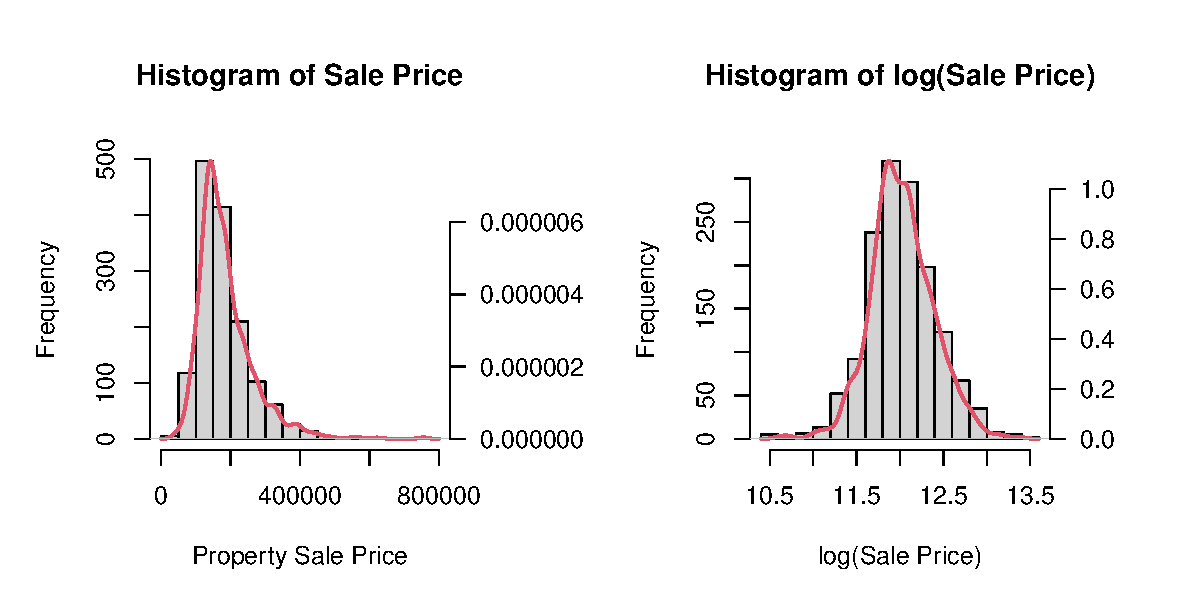
\includegraphics{STAT-444-FINAL-PROJECT-PROPOSAL_files/figure-latex/unnamed-chunk-5-1.pdf}
\caption{Histograms of the response variable, Sale Price\label{}}
\end{figure}

\hypertarget{correlations-with-the-dependent-variable}{%
\subsection{Correlations with the dependent
variable}\label{correlations-with-the-dependent-variable}}

\begin{itemize}
\tightlist
\item
  Based on our correlation analysis, the five numeric variables with the
  highest correlations with our dependent variable are: \vspace{0.2cm}

  \begin{itemize}
  \tightlist
  \item
    Overall.Qual: Rates the overall material and finish of the house.
  \item
    Gr.Liv.Area: Above grade (ground) living area square feet.
  \item
    Garage.Cars: Size of garage in car capacity.
  \item
    Garage.Area: Size of garage in square feet.
  \item
    Total.Bsmt.SF: Total square feet of basement area.
  \end{itemize}
\end{itemize}

\hypertarget{check-if-there-is-a-high-degree-of-correlation-or-linear-association-among-independent-variables}{%
\subsection{Check if there is a high degree of correlation or linear
association among independent
variables}\label{check-if-there-is-a-high-degree-of-correlation-or-linear-association-among-independent-variables}}

\begin{itemize}
\tightlist
\item
  Some independent variables are strongly correlated; this behavior is
  to be expected, as some covariates provide similar information.
  \vspace{0.2cm}

  \begin{itemize}
  \tightlist
  \item
    For example, the high correlation between the variable
    \textbf{Garage Area} (size of garage in square feet) and
    \textbf{Garage Cars} (size of garage in car capacity) is not
    surprising.
  \item
    To address such redundant pairs, we will select one covariate from
    each pair, excluding the other from the analysis.
  \end{itemize}
\end{itemize}

\begin{figure}
\centering
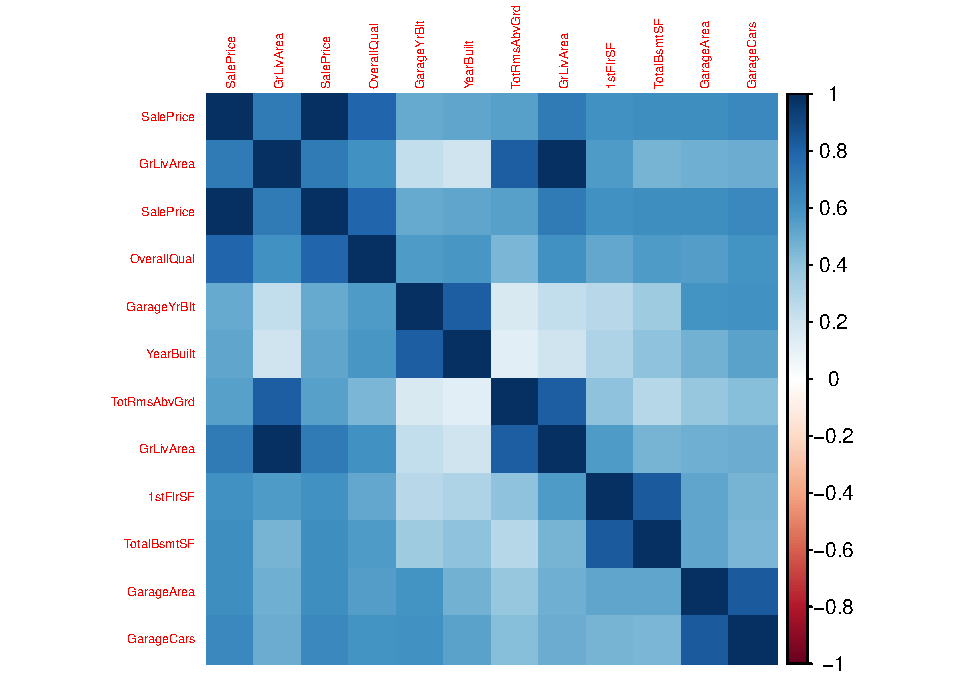
\includegraphics{STAT-444-FINAL-PROJECT-PROPOSAL_files/figure-latex/unnamed-chunk-8-1.pdf}
\caption{Correlation matrix of independent variables\label{}}
\end{figure}

\hfill\break

\hypertarget{other-interesting-but-non-numeric-variables}{%
\subsection{Other interesting but non-numeric
variables}\label{other-interesting-but-non-numeric-variables}}

\hfill\break
\hfill\break
We note some non-numeric variables of interest below.

\begin{itemize}
    \item \textbf{Neighborhood.} There appears to be a significant difference in the average property sale price by neighborhood.
\vspace{0.2cm}
\item The dataset contains several categorical variables with low variance (i.e. near-constant), which likely hold negligible predictive power, including:
\vspace{0.2cm}
\begin{itemize}
    \item \texttt{Street} - type of road access to property
    \item \texttt{Utilities} - type of utilities available
    \item \texttt{Roof.Matl} - roof material
\end{itemize}
\end{itemize}

\begin{figure}
\centering
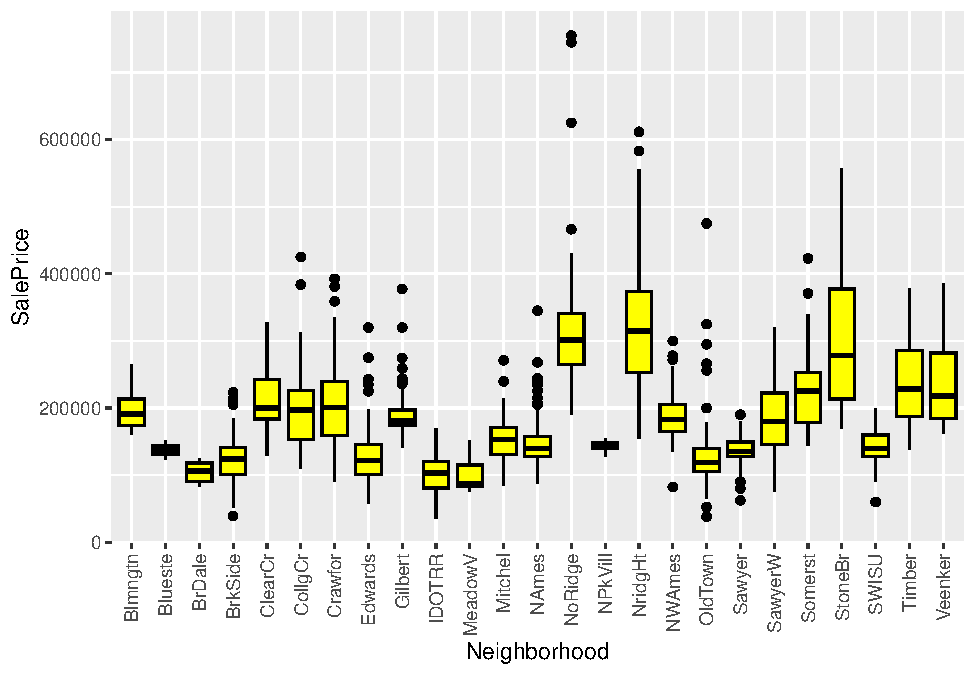
\includegraphics{STAT-444-FINAL-PROJECT-PROPOSAL_files/figure-latex/unnamed-chunk-9-1.pdf}
\caption{Boxplot showing the distribution of SalePrice across
Neighborhood\label{}}
\end{figure}

\hypertarget{plan}{%
\section{Plan}\label{plan}}

The objective of this study is to determine the viability and
effectiveness of employing additive models, splines, and polynomial
regression for predicting house prices. We focus our attention on the
following:

\begin{itemize}
\item
  \textbf{Accuracy}: Assess the predictive accuracy of additive models,
  splines, and polynomial regression in comparison to traditional
  regression models commonly used in the real estate domain.
    \vspace{0.2cm}
\item
  \textbf{Flexibility}: Analyze the ability of these techniques to
  capture complex relationships between house price predictors, such as
  square footage, location, number of bedrooms, and other relevant
  features.
  \vspace{0.2cm}
\item
  \textbf{Interpretability}: Evaluate the interpretability and
  explainability of the models, ensuring that the predictions can be
  easily understood and justified by stakeholders.
  \vspace{0.2cm}
\end{itemize}

To achieve our objective, we propose the following methodology as an
outline:

\begin{enumerate}
\item
  \textbf{Initial Benchmark}: Use the performance of linear regression, with simple categorical encoding, on the full
  feature set as an initial benchmark.
  \vspace{0.2cm}
\item
  \textbf{Data Preprocessing}: Handle missing/invalid values and outliers and perform feature engineering to enhance
  the models' predictions. To mitigate the ``curse of dimensionality" and reduce collinearity in the dataset, we
   will use a low variance filter and clustering techniques such as Principal Component Analysis (PCA).
   \vspace{0.2cm}
\item
  \textbf{Model Implementation}: Develop additive models, splines, and
  polynomial regression models using appropriate algorithms and
  frameworks, such as generalized additive models (GAMs) and polynomial
  regression libraries in R. We will also apply penalization techniques
  to prevent overfitting (e.g. forward/backward selection, LASSO/Ridge regression)
  while including interactions between covariates to model any non-linear relationships.
  \vspace{0.2cm}
\item
  \textbf{Model Evaluation}: Assess the performance of the models using
  appropriate evaluation metrics, such as mean squared error (MSE), root
  mean squared error (RMSE), and R-squared values and compare the
  results with benchmark models.
  \vspace{0.2cm}
\item
  \textbf{Interpretation and Explainability}: Examine the contributions of each
  feature and the underlying relationships identified by the models. Visualize the results in an intuitive yet
  comprehensive manner.
\end{enumerate}

\bibliographystyle{imsart-nameyear}
\bibliography{ims.bib}


\end{document}
